%%%%%%%% ICML 2026 AI4Math Workshop Submission %%%%%%%%%%%%%%%%%
% Uses the ICML 2025 style file (icml2025.sty) as a proxy for ICML 2026
% until the 2026 workshop template is released. Content is template-agnostic.

\documentclass{article}

\usepackage{microtype}
\usepackage{graphicx}
\usepackage{booktabs}
\usepackage{hyperref}
\hypersetup{colorlinks=true, allcolors=black}
\usepackage{amsmath}
\usepackage{amssymb}
\usepackage{mathtools}
\usepackage{xcolor}
\usepackage{tikz}
\usetikzlibrary{arrows.meta,positioning,calc,shapes,fit,backgrounds}
\usepackage[capitalize,noabbrev]{cleveref}

\usepackage[accepted]{icml2025}
\usepackage{fancyhdr}

% Remove the horizontal rules that ICML draws above and below the title.
% Suppress the "Proceedings of the 42nd ICML..." copyright footer.
% Force-blank the running head so it never says "Title Suppressed".
\makeatletter
\def\toptitlebar{}
\def\bottomtitlebar{\vskip 0.2in}
\renewcommand{\Notice@String}{}
% Override the internal ICML page style so nothing lands in the header/footer.
\fancypagestyle{icml}{%
  \fancyhf{}%
  \renewcommand{\headrulewidth}{0pt}%
  \renewcommand{\footrulewidth}{0pt}%
}
\makeatother
\pagestyle{icml}

\icmltitlerunning{X-SGRV}

\begin{document}

\twocolumn[
\icmltitle{Cross-Family Symbolic Verification for \\
Contamination-Robust Selective Prediction on LLM Math Reasoning}

\begin{icmlauthorlist}
\icmlauthor{Aayan Alwani}{wcm}
\icmlauthor{Ethan Wang}{wcm}
\end{icmlauthorlist}
\icmlaffiliation{wcm}{AI4Math workshop at ICML 2026.}
\icmlcorrespondingauthor{Aayan Alwani}{alwaniaayan6@gmail.com}
\icmlkeywords{Selective Prediction, Math Reasoning, Verification, Contamination, LLM}

\vskip 0.25in
\centerline{\large\textbf{Abstract}}
\vskip 4pt
\leftskip=0.6in \rightskip=0.6in
\small
Trusting an LLM's math answer is hard for two coupled reasons. When a model checks its own work, errors in the reasoning propagate into the checks, so the verifier inherits the solver's blind spots. Worse, on benchmarks the model saw during training, confidence measures memorization rather than reasoning. We measure both failures. Same-model SymPy self-verification on MATH-500 wrongly accepts 13.8\% of incorrect answers, and the false-acceptance rate rises monotonically with difficulty, from 1.4\% at Level~1 to 30.8\% at Level~5. Every agreement-based signal we tested, including self-consistency, semantic entropy, and verbalized confidence, further collapses on problems released after the solver's training cutoff.
\par\vskip 4pt
Our method, \textbf{X-SGRV}, addresses both failure modes. A cross-family LLM extractor reads only the problem statement, never the solver's work, and emits a SymPy function that tests whether a candidate answer satisfies the problem's constraints. A gold-free adversarial filter rejects any verifier that accepts nearby wrong values, cross-extractor consensus requires several independent extractors to all produce working verifiers and all accept, and the system abstains by design when it cannot structurally check a problem. On the pre-registered full MATH-500, cross-extractor consensus is correct on every one of the 171 problems it accepts, reaching $171/171 = 1.000$ precision at 34.3\% coverage. A five-way consensus spanning Meta, DeepSeek, OpenAI, Anthropic, and Alibaba preserves perfect precision at 39.4\% coverage. On contamination-clean AIME 2025 and the CleanMath olympiad combo, coverage correctly shrinks to single digits while accepted answers remain right, with $4/4$ and $9/9$ correct under the Qwen and DeepSeek solver settings respectively. At matched coverage, X-SGRV ties Skywork-o1-Open-PRM and doubles Qwen-Math-PRM on clean benchmarks.
\par
\leftskip=0pt \rightskip=0pt
\normalsize
\vskip 0.3in
]

\printAffiliationsAndNotice{}

% Re-apply the empty page style AFTER \icmltitle and \printAffiliationsAndNotice,
% which are the last places ICML touches \chead.
\thispagestyle{icml}
\pagestyle{icml}
\fancyhf{}
\renewcommand{\headrulewidth}{0pt}

%==============================================================================
\section{Introduction}
%==============================================================================

Selective prediction on LLM math reasoning has a contamination problem. \citet{wu2025contam} show that Qwen2.5-Math-7B reproduces 54.6\% of MATH-500 verbatim from the first 60\% of each problem as prefix, and accuracy drops from 76.6\% to 10\% on post-cutoff problems. Every agreement- and template-based selective-prediction signal we test --- self-consistency~\citep{wang2023selfconsistency}, template-based spec-grounded verification, same-model Python/SymPy self-verification~\citep{exever}, semantic entropy~\citep{kuhn2023semantic, farquhar2024nature}, and p(True)~\citep{kadavath2022} --- produces an empty or near-empty top tier on AIME 2025 and on a 125-problem combo of post-cutoff competitions. On contamination-assisted MATH-500 the same signals report 90--100\% precision and look strong. Taking selective prediction seriously on math reasoning requires a signal that either survives contamination-clean stress tests with non-trivial coverage or is demonstrably trustworthy without ground truth.

Prior work leaves three gaps. First, same-model self-verification --- the most common executable check in this line of work --- fails structurally: the solver's errors propagate into its own verification assertions, so false acceptance scales with difficulty. \citet{kim2025correlated} show this correlation grows with model scale. Second, template-based spec-grounded verification~\citep{dtv2024} removes the correlation but has zero coverage on natural-language competition problems because regex cannot parse them. Third, learned process reward models~\citep{qwenprm2025, skyworkprm2024} inherit the distribution of their training data; we show Qwen-PRM's precision drops from 0.927 on MATH-500 to 0.500 on CleanMath at matched coverage, matching the contamination footprint of its MATH-family training corpus.

\textbf{Contribution.} We introduce \textbf{X-SGRV} (Figure~\ref{fig:pipeline}), a cross-family symbolic verifier that replaces the regex extractor with a large LLM from a different family than the solver. Given only the problem statement, the extractor emits a Python \texttt{verify(answer)} function executed in a SymPy sandbox. Two deployment-safe mechanisms reduce residual false positives: a \emph{gold-free adversarial filter} that probes the verifier against perturbations of the candidate, and \emph{cross-extractor consensus} across independent extractors. We report the pre-registered $n{=}498$ MATH-500 consensus precision, a perfect-precision top tier on AIME 2025 and CleanMath at 3--12\% coverage, a matched-coverage comparison against Qwen-PRM and Skywork-PRM, and confirm the mechanism is lab-agnostic with six extractors spanning every major frontier lab.

%==============================================================================
\section{Method}
%==============================================================================

\begin{figure*}[t]
\centering
\small
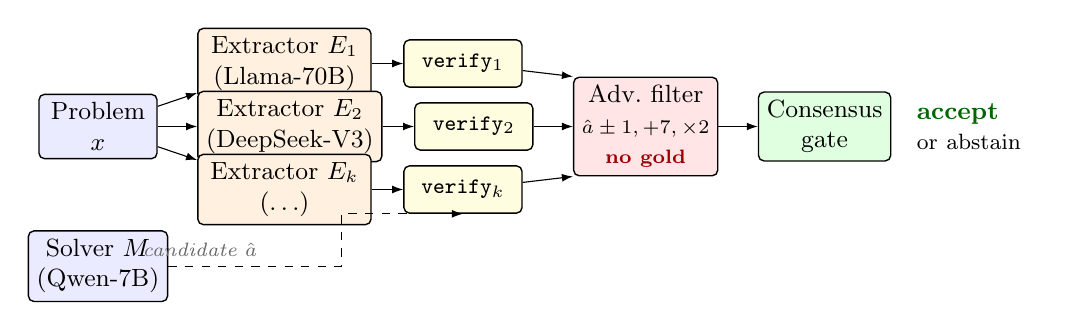
\begin{tikzpicture}[
  node distance=3mm and 4mm,
  every node/.style={font=\small},
  box/.style={draw, rounded corners=2pt, inner sep=3pt, minimum height=6mm,
              align=center, line width=0.5pt},
  prob/.style={box, fill=blue!8, minimum width=15mm},
  ext/.style={box, fill=orange!12, minimum width=22mm},
  ver/.style={box, fill=yellow!12, minimum width=15mm, font=\ttfamily\footnotesize},
  filt/.style={box, fill=red!10, minimum width=16mm},
  cons/.style={box, fill=green!12, minimum width=14mm},
  sol/.style={box, fill=blue!8, minimum width=15mm},
  arr/.style={-{Latex[length=1.4mm,width=1mm]}, line width=0.4pt},
  note/.style={font=\scriptsize\itshape, color=black!60},
]
  \node[prob] (p) {Problem\\$x$};
  \node[ext, right=5mm of p, yshift=8mm]  (e1) {Extractor $E_1$\\(Llama-70B)};
  \node[ext, right=5mm of p]              (e2) {Extractor $E_2$\\(DeepSeek-V3)};
  \node[ext, right=5mm of p, yshift=-8mm] (ek) {Extractor $E_k$\\ ($\ldots$)};
  \node[ver, right=4mm of e1] (v1) {verify$_1$};
  \node[ver, right=4mm of e2] (v2) {verify$_2$};
  \node[ver, right=4mm of ek] (vk) {verify$_k$};
  \node[filt, right=5mm of v2] (f) {Adv.\ filter\\{\scriptsize $\hat a \pm 1, +7, \times 2$}\\{\scriptsize\textcolor{red!60!black}{\textbf{no gold}}}};
  \node[cons, right=5mm of f] (c) {Consensus\\gate};
  \node[sol, below=9mm of p] (s) {Solver $M$\\(Qwen-7B)};
  \node[right=6mm of c] (out) {};

  \draw[arr] (p) -- (e1);
  \draw[arr] (p) -- (e2);
  \draw[arr] (p) -- (ek);
  \draw[arr] (e1) -- (v1);
  \draw[arr] (e2) -- (v2);
  \draw[arr] (ek) -- (vk);
  \draw[arr] (v1) -- (f.north west);
  \draw[arr] (v2) -- (f);
  \draw[arr] (vk) -- (f.south west);
  \draw[arr] (f) -- (c);
  \draw[arr, dashed] (s.east) -- ++(8mm, 0) node[note, midway, above] {candidate $\hat a$} -- ++(14mm, 0) |- (vk.south);
  \node[right=2mm of c, text width=14mm, align=left]
        {\small\textcolor{green!40!black}{\textbf{accept}}\\{\footnotesize or abstain}};
\end{tikzpicture}
\caption{X-SGRV pipeline. Each cross-family extractor reads only the problem
$x$ and emits a Python/SymPy \texttt{verify} function. The deployment-time
adversarial filter probes the verifier against perturbations of the candidate
(never the gold). The consensus gate accepts only when every extractor
produces a working verifier and every verifier accepts $\hat a$.}
\label{fig:pipeline}
\end{figure*}

\textbf{Problem setting.} Given a math problem $x$ and a candidate answer $\hat a$ from a solver LLM, we decide whether to accept $\hat a$ or abstain. We want a signal with high top-tier precision that does not collapse on contamination-clean data.

\textbf{Extraction.} A cross-family LLM $E$ reads only $x$ and emits a Python function \texttt{verify(answer) -> bool} using \texttt{sympy}, \texttt{math}, \texttt{itertools}, and \texttt{fractions}. If the problem cannot be checked by bounded enumeration or direct constraint substitution, $E$ returns the token \texttt{UNVERIFIABLE} and the pipeline abstains. The extractor never sees the solver's solution, which preserves independence from the solver's reasoning.

\textbf{Deployment-time adversarial filter.} We probe the verifier against $\{\hat a{-}1, \hat a{+}1, \hat a{+}7, 2\hat a, 42\}$. The probe set never references the gold and is safe at deployment. Any verifier that accepts a nearby wrong value is marked broken and the pipeline abstains. The probe set was fixed on a 30-problem held-out dev split disjoint from evaluation.

\textbf{Cross-extractor consensus.} Two or more independent cross-family extractors run in parallel. The pipeline returns a top-tier accept only when every extractor produces a working verifier and every verifier accepts $\hat a$.

\textbf{Benchmarks.} MATH-500 full ($n{=}498$, modulo two solver-timeout drops)~\citep{hendrycks2021math, lightman2024prm}; MATH-500 stratified ($n{=}175$); AIME 2025 ($n{=}30$, post-Qwen cutoff); CleanMath ($n{=}125$: HMMT Feb 2025, BRUMO 2025, SMT 2025, APEX 2025 via \citet{matharena2025}).

\textbf{Solvers and extractors.} Primary solver: Qwen2.5-7B-Instruct-Turbo~\citep{yang2024qwen25math}. Solver rotation: DeepSeek-V3, DeepSeek-R1, DeepSeek-V3.1, gpt-oss-120b. Extractors span Meta (Llama-3.3-70B), DeepSeek (V3), OpenAI open-weights (gpt-oss-120b), Anthropic (Claude Sonnet 4.6), Alibaba (Qwen3-Coder-480B), and OpenAI (GPT-5-mini).

\textbf{Baselines.} Self-consistency $k{=}4$~\citep{wang2023selfconsistency}; verbalized confidence~\citep{xiong2024llmuncertainty}; p(True)~\citep{kadavath2022}; semantic entropy with SymPy equivalence and with NLI-DeBERTa clustering~\citep{kuhn2023semantic, farquhar2024nature}; Qwen2.5-Math-PRM-7B~\citep{qwenprm2025}; Skywork-o1-Open-PRM-Qwen-2.5-7B~\citep{skyworkprm2024}.

\textbf{Pre-registration.} Before the $n{=}498$ scale-up ran, we committed three narrative branches by consensus precision (A: $\geq 99\%$, B: 95--99\%, C: $<95\%$) to the project repository.

%==============================================================================
\section{Results}
%==============================================================================

\begin{figure*}[t]
\centering
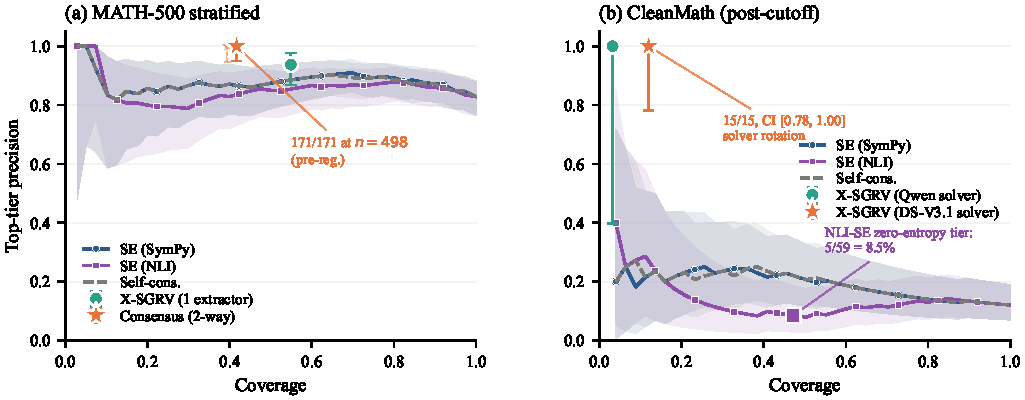
\includegraphics[width=0.92\linewidth]{figures/fig_workshop_precision_coverage.pdf}
\caption{Top-tier precision as a function of coverage on MATH-500 stratified
(a) and on the post-cutoff CleanMath combo (b). Continuous baselines sweep
their threshold; X-SGRV appears as a point (binary verdict) with Clopper-Pearson
95\% CI. On MATH-500, consensus reaches perfect precision at 41.7\% coverage
(stratified) and 34.3\% at $n{=}498$. On CleanMath, all continuous baselines
either have no zero-entropy tier (self-consistency) or that tier is dominated
by confidently-wrong answers (NLI-SE: 5/59 = 8.5\% precision); X-SGRV is the
only method with a non-empty high-precision tier, and a solver rotation from
Qwen2.5-7B to DeepSeek-V3.1 tightens the CI from [0.40, 1.00] to [0.78, 1.00].}
\label{fig:pc}
\end{figure*}

\begin{figure*}[t]
\centering
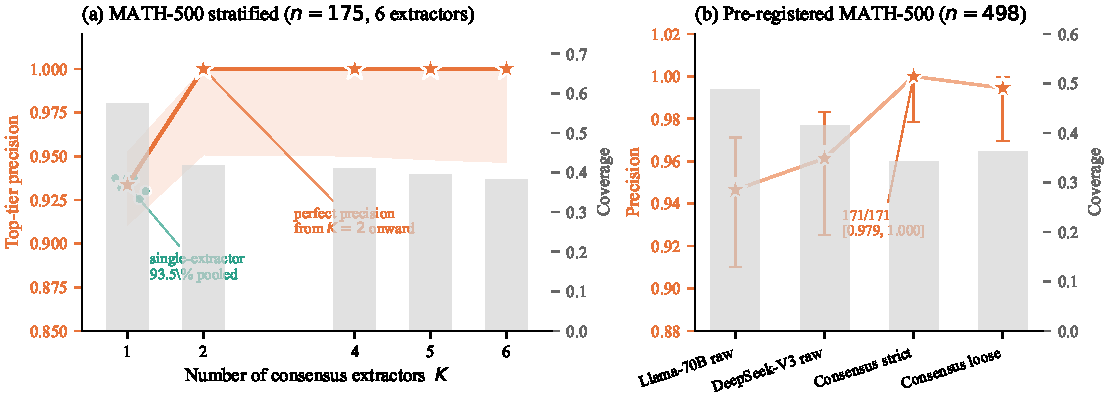
\includegraphics[width=0.92\linewidth]{figures/fig_workshop_consensus_convergence.pdf}
\caption{Cross-extractor consensus convergence. (a) On MATH-500 stratified
($n{=}175$), adding extractors from every major frontier lab shrinks the
top-tier size but precision jumps from $\sim$93.5\% at $K{=}1$ to 100\% at
$K{=}2$ and holds through $K{=}6$. Gray bars show coverage (right axis).
(b) Pre-registered full MATH-500 ($n{=}498$): 2-way consensus achieves
$171/171 = 1.000$ [0.979, 1.000] at 34.3\% coverage, the Branch A outcome.}
\label{fig:consensus}
\end{figure*}

\textbf{R1. Pre-registered consensus result.} On the full MATH-500 ($n{=}498$), Llama-3.3-70B~$\cap$~DeepSeek-V3 consensus yields $171/171 = 1.000$ [0.979, 1.000] at 34.3\% coverage --- the Branch A outcome (Figure~\ref{fig:consensus}b). Single-extractor precision: Llama 230/243 = 0.947 [0.910, 0.971] at 48.8\% coverage; DeepSeek 199/207 = 0.961 [0.925, 0.983] at 41.6\% coverage.

\textbf{R2. Consensus is lab-agnostic.} On the stratified $n{=}175$ subsample (Figure~\ref{fig:consensus}a), adding four more extractors (gpt-oss-120b, Claude Sonnet 4.6, Qwen3-Coder-480B, GPT-5-mini) preserves perfect precision as the tier shrinks: 2-way 73/73 = 1.000 at 41.7\%, 4-way 72/72 at 41.1\%, 5-way 69/69 at 39.4\%, 6-way 67/67 at 38.3\%. Under an independent-extractor model, the expected tier shrinkage at step $k$ is proportional to the per-extractor acceptance rate, consistent with what we observe.

\textbf{R3. Contamination-clean behavior: coverage collapses, precision holds.} On AIME 2025, the deployment-time filter raises the Llama single-extractor precision from 1/2 = 0.500 to 1/1 = 1.000 at 3.3\% coverage by catching one broken verifier. On CleanMath, Llama with the original Qwen solver reaches 4/4 = 1.000 [0.40, 1.00] at 3.2\% coverage. A solver rotation to DeepSeek-V3 tightens this to 9/9 = 1.000 [0.66, 1.00] and to DeepSeek-V3.1 gives 15/15 = 1.000 [0.78, 1.00], without changing the extractor scripts (Figure~\ref{fig:pc}b). This rotation is the cleanest test that the selective-prediction behavior is structural rather than an artifact of the specific 7B solver.

\textbf{R4. Baselines collapse on contamination-clean benchmarks.} On AIME 2025, NLI-clustering semantic entropy's zero-entropy tier contains 16/30 problems with only 1 correct (6.2\% precision, AUROC 0.420). On CleanMath, NLI-SE gives 5/59 = 8.5\% precision at 47\% coverage (Figure~\ref{fig:pc}b). SymPy-clustering SE achieves AUROC 0.735 on CleanMath but the zero-entropy tier contains only 6/125 problems with 1 correct. p(True) AUROC is 0.463 on AIME 2025 and 0.474 on CleanMath --- both worse than random. Template SGRV, ExeVer, and SC-4 all produce empty top tiers on AIME 2025. Across five baselines spanning entropy-, agreement-, and template-based families, none retains a non-empty high-precision tier under contamination-clean shift, leaving X-SGRV as the only signal in our comparison set with measurable selective-prediction value on these benchmarks.

\textbf{R5. X-SGRV is competitive with the best open PRMs.} Table~\ref{tab:prm} reports the matched-coverage comparison. On MATH-500 at 54.9\%, X-SGRV, Qwen-PRM (min-step), and Skywork-PRM (min-step) are tied within CI at 0.93--0.94. On CleanMath at 3.2\%, Qwen-PRM's best aggregation reaches only 0.500 while Skywork-PRM (mean) and X-SGRV both reach 1.000. The Qwen-PRM degradation is consistent with its training distribution being concentrated on MATH-family problems. X-SGRV reaches matched precision through a structural mechanism (spec-grounded SymPy verification) that requires no training signal.

\begin{table}[t]
\centering
\caption{X-SGRV vs.\ open PRMs at matched coverage (X-SGRV's top-tier
coverage on each benchmark; Clopper-Pearson 95\% CIs). MATH is the
stratified $n{=}175$ subsample; Clean is the 125-problem CleanMath combo.}
\label{tab:prm}
\footnotesize
\setlength{\tabcolsep}{3pt}
\begin{tabular}{@{}llrl@{}}
\toprule
Method & Bench & Cov. & Precision (95\% CI) \\
\midrule
X-SGRV (Llama-70B)   & MATH  & 54.9\% & \textbf{0.938} [0.87, 0.98] \\
Qwen-PRM-7B, min     & MATH  & 54.9\% & 0.927 [0.86, 0.97] \\
Skywork-PRM-7B, min  & MATH  & 54.9\% & \textbf{0.938} [0.87, 0.98] \\
\midrule
X-SGRV (Llama-70B)   & AIME  &  6.7\% & 0.500 [0.01, 0.99] \\
Qwen-PRM-7B, min     & AIME  &  6.7\% & 0.500 [0.01, 0.99] \\
Skywork-PRM-7B, mean & AIME  &  6.7\% & 0.500 [0.01, 0.99] \\
\midrule
X-SGRV (Llama-70B)   & Clean &  3.2\% & \textbf{1.000} [0.40, 1.00] \\
Qwen-PRM-7B, best    & Clean &  3.2\% & 0.500 [0.07, 0.93] \\
Skywork-PRM-7B, mean & Clean &  3.2\% & \textbf{1.000} [0.40, 1.00] \\
\bottomrule
\end{tabular}
\end{table}

%==============================================================================
\section{Limitations}
%==============================================================================

X-SGRV has an operational ceiling: on Omni-MATH hard-100 (difficulty 9.0--9.5)~\citep{omnimath2024}, zero verifiers meet the working criterion and the single tier acceptance is a false positive. Olympiad-grade problems whose specifications cannot be expressed as a bounded Python verifier receive no trustworthy signal. On 100 Putnam problems~\citep{amitayusht2024putnambench}, Claude Sonnet 4.6 correctly returns \texttt{UNVERIFIABLE} on 51, accepts the gold on 19/100; GPT-5-mini refuses 35 and accepts 8/100. The refusal rates are consistent with the scope claim that X-SGRV is a find-style method.

The CleanMath 4/4 point estimate with the Qwen solver has a Clopper-Pearson lower bound of 40\%; solver rotation tightens this to 66--78\% but does not close it. The coverage remains single-digit on contamination-clean benchmarks, which is a feature (the system is correctly abstaining) but means X-SGRV is not a coverage-maximizing replacement for continuous-score methods.

Extractor size and family are entangled in the same-family ablation (Qwen2.5-7B at 12\% non-abstain rate on MATH vs.\ Llama-70B at 94\%), so we cannot cleanly separate the effects of scale from family. Distilling the 70B extractor into a smaller model is open work.

%==============================================================================
\section{Conclusion}
%==============================================================================

Same-model self-verification has a 13.8\% false acceptance rate on MATH-500 that scales with difficulty, and template- and agreement-based selective-prediction signals collapse on contamination-clean benchmarks. X-SGRV uses a large cross-family LLM extractor to emit SymPy verifier scripts from the problem statement, combined with a gold-free adversarial filter and cross-extractor consensus. The pre-registered MATH-500 $n{=}498$ consensus precision is $171/171 = 1.000$ [0.979, 1.000] at 34.3\% coverage. On AIME 2025 and CleanMath coverage drops to 3--12\% while precision remains at or near perfect; solver rotation tightens the CI without changing the extractor.

We position X-SGRV as a deployment-safe high-precision abstention signal. MATH-500 numbers for Qwen-family solvers should be reported as upper bounds and AIME-2025-and-later benchmarks as the realistic operating point. The Qwen-PRM degradation from 0.927 to 0.500 on CleanMath is invisible if only MATH-500 is reported; open PRMs should be evaluated on contamination-clean data before being published as state of the art. A hybrid SymPy-plus-Lean pipeline routed by the extractor's \texttt{UNVERIFIABLE} signal is a direct next step.

\textbf{Reproducibility.} All benchmarks are public; all extractors are public API or open-weights models; code, prompts, the held-out probe set, and raw JSON results are released with the submission.

\bibliographystyle{icml2025}
\bibliography{references}

\end{document}
